% 
% PARTIE 3
% 
\section{Étude du comportement sur terrain accidenté \label{sec_3}}

\ifprof
\else

Le terrain volcanique est en pratique très accidenté, avec la présence d'obstacles (roches) et de
fortes pentes (\autoref{fig_10}). Par conséquent, le système de locomotion de ROBOVOLC doit être
adapté à ce type de terrain.
\fi

\begin{obj}
L'objectif de cette partie est de valider les performances d'agilité et de franchissement
d'obstacle du système sur des terrains non structurés avec difficultés topologiques
(pentes, obstacles). On souhaite vérifier les critères suivants du cahier des charges :
\begin{center}
\begin{tabular}{ll}
\hline
\textbf{Critère} & \textbf{Valeur} \\ \hline \hline
Masse maximale des composants modulaires & \SI{200}{kg}\\ \hline
Pente maximale du sol & 40\degres \\ \hline
Hauteur maximale d'un obstacle & \SI{400}{mm} \\ 
\hline
\end{tabular}
\end{center}
\end{obj}


\ifprof
\else

Dans toute cette partie, les effets dynamiques sont négligés et on se place en statique.


\begin{figure}[H]
\centering
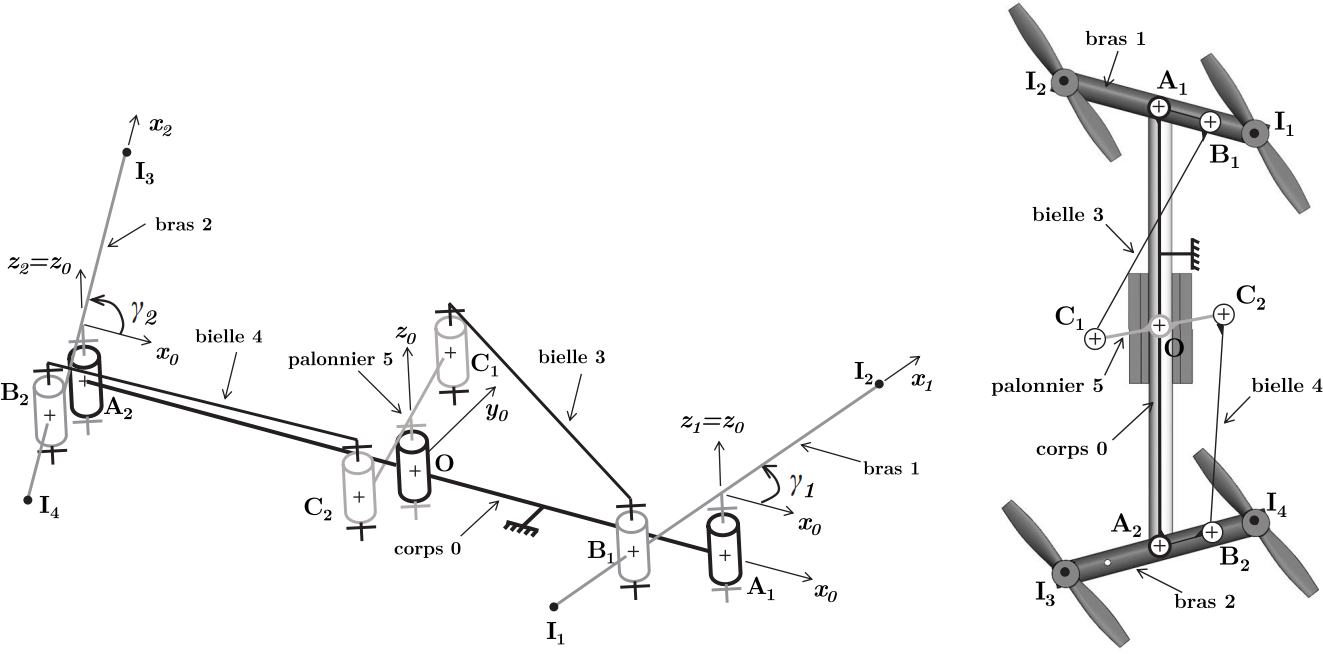
\includegraphics[width=.45\linewidth]{fig_10.png}
\caption{Illustration du comportement de ROBOVOLC sur terrain accidenté \label{fig_10}}
\end{figure}
\fi



%\subsection{Modélisation du châssis}
%
%\begin{obj}
%Dans cette sous-partie, on établit un modèle statique du châssis de ROBOVOLC.
%\end{obj}
%
%La mobilité sur terrain accidenté est obtenue, en plus de par la motorisation indépendante des
%roues, par l'utilisation d'un châssis articulé. Celui-ci a une structure tubulaire avec des articulations
%passives (non actionnées) permettant à ROBOVOLC de s'adapter à toute surface non plane. Une
%illustration des cinq mouvements indépendants permis par les articulations est donnée sur la
%\autoref{fig_11}.
%
%\begin{figure}[H]
%\centering
%\begin{tabular}{|p{.3\linewidth}|p{.3\linewidth}|p{.3\linewidth}|}
%\hline
%Châssis au repos & Mouvement 1 : rotation de l'essieu avant
%autour de l'axe longitudinal & Mouvement 2 :
%rotation de l'essieu central
%autour de l'axe longitudinal \\ \hline
%\begin{center}
%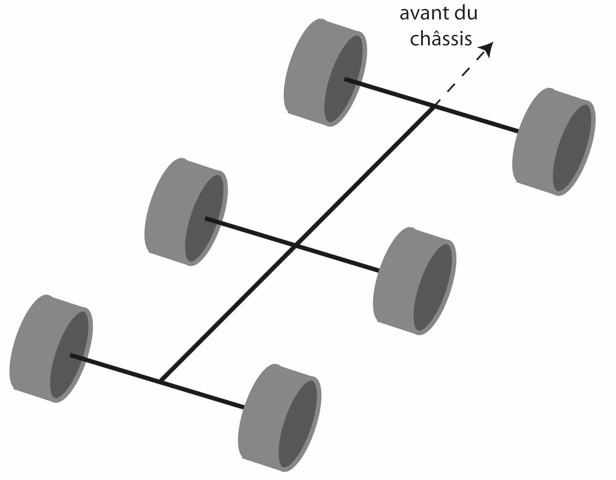
\includegraphics[width=.9\linewidth]{fig_11_a.png}
%\end{center}
%&
%\begin{center}
%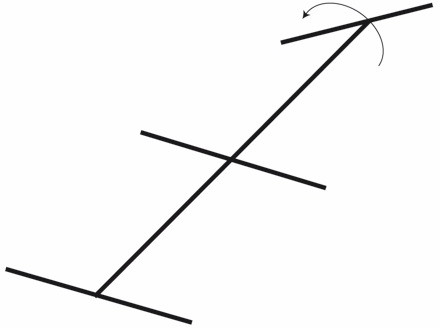
\includegraphics[width=.9\linewidth]{fig_11_b.png}
%\end{center}
%&
%\begin{center}
%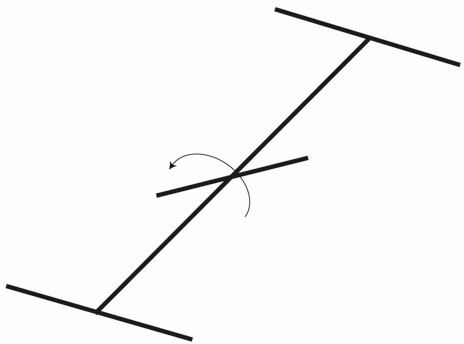
\includegraphics[width=.9\linewidth]{fig_11_c.png}
%\end{center} \\ \hline
%Mouvement 3 :
%rotation de l'essieu arrière
%autour de l'axe longitudinal & 
%Mouvement 4 :
%rotation de l'arbre avant
%autour de l'axe transversal &
%Mouvement 5 :
%rotation de l'arbre arrière
%autour de l'axe transversal \\ \hline
%\begin{center}
%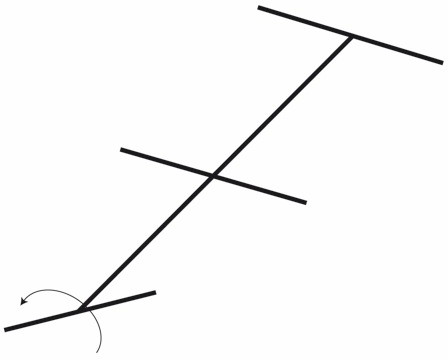
\includegraphics[width=.9\linewidth]{fig_11_d.png}
%\end{center}
%&
%\begin{center}
%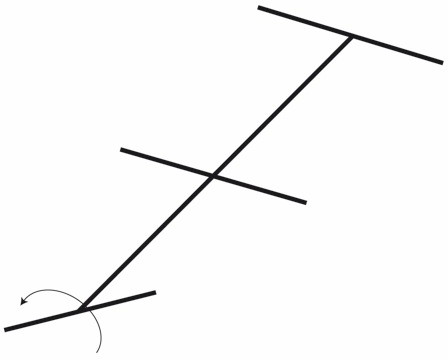
\includegraphics[width=.9\linewidth]{fig_11_e.png}
%\end{center}
%&
%\begin{center}
%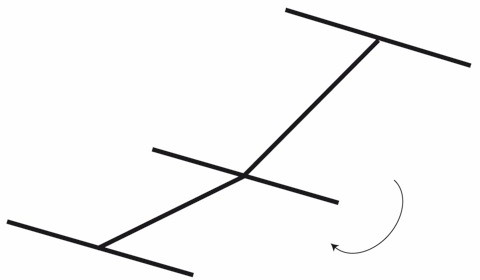
\includegraphics[width=.9\linewidth]{fig_11_f.png}
%\end{center} \\ \hline
%\end{tabular}
%
%\caption{Illustration des mouvements de déformation du châssis\label{fig_11}}
%\end{figure}
%
%Le châssis est composé de cinq parties orientables les unes par rapport aux autres (\autoref{fig_12}) :
%\begin{itemize}
%\item l'essieu avant, noté EAV, reliant les roues avant 1 et 2 ;
%\item l'essieu central, noté EC, reliant les roues centrales 3 et 4 ;
%\item l'essieu arrière, noté EAR, reliant les roues arrière 5 et 6 ;
%\item l'arbre avant, noté AAV, connectant les essieux EAV et EC ;
%\item l'arbre arrière, noté AAR, connectant les essieux EC et EAR.
%\end{itemize}
%On rappelle que l'empattement entre deux essieux successifs est noté $a$, et que la distance entre
%deux roues d'un même essieu est notée $2e$.
%Les différentes parties sont reliées entre elles par des articulations possédant une raideur en
%rotation imposée. Par la suite, on supposera cette raideur négligeable devant les autres actions
%mécaniques mises en jeu.
%Un schéma cinématique de la plateforme (châssis+roues) est présenté sur la \autoref{fig_12}.
%
%\begin{figure}[H]
%\centering
%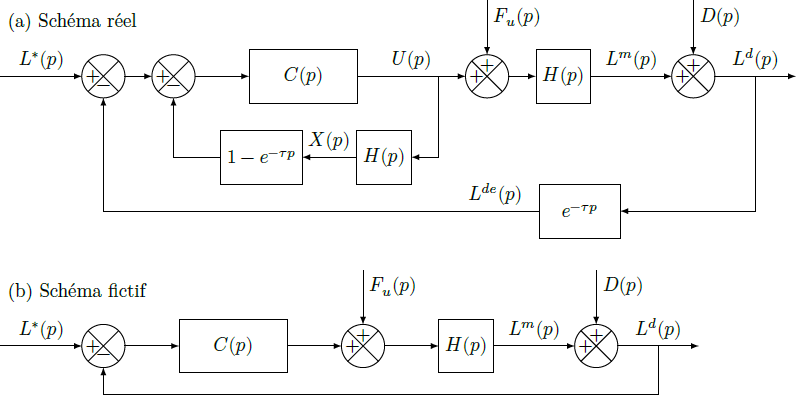
\includegraphics[width=.45\linewidth]{fig_12.png}
%\caption{Schéma cinématique de la plateforme\label{fig_12}}
%\end{figure}
%
%Les deux articulations EC-AAV et EC-AAR, situées à une distance longitudinale $\pm b$ de l'essieu
%EC, autorisent une rotation selon les directions $\vect{x}$ et $\vect{y}$; elles sont modélisées par des liaisons
%rotule à doigt de centres respectifs $B$ et $C$. Les deux articulations EAV-AAV et EAR-AAR
%autorisent une rotation selon la direction $\vect{x}$ seulement ; elles sont modélisées par des liaisons
%pivot d'axe $\axe{O}{x}$.
%
%D'autre part, les six liaisons essieu-roue sont modélisées par des liaisons pivot d'axe $\axe{A}{y}$
%(roues avant), $\axe{O}{y}$ (roues centrales) ou $\axe{D}{y}$ (roues arrière). De plus, le contact de chaque
%roue i avec le sol est modélisé en première approche par une liaison ponctuelle de normale
%$\axe{P_i}{z}$.
%
%On considère dans les questions \ref{q3.1} et \ref{q3.2} que les liaisons sont parfaites sans frottements.
%
%
%\question{ \label{q3.1} Déterminer le nombre de mobilités du modèle du système.}
%
%\question{ \label{q3.2} Montrer que le modèle est isostatique. Conclure quant à la capacité du châssis à maintenir
%les roues au contact du sol en toute circonstance.}
%
%\question{ \label{q3.3} Proposer un modèle de liaison parfaite pour le contact roue-sol qui permet de tenir compte,
%dans une étude de statique sans glissement, du frottement longitudinal et transversal. Peut-on
%calculer toutes les inconnues statiques de liaison dans ce cas ?}
%
%
%On considère par la suite que le sol est horizontal dans la direction $\vect{y}$; on se ramène alors à un
%problème dans le plan médian $\left(O,\vect{x},\vect{z}\right)$. Dans cette configuration plane, la plateforme est
%constituée de trois ensembles articulés pour s'adapter au terrain accidenté (\autoref{fig_13}) :
%\begin{itemize}
%\item l'ensemble avant (noté ENSAV) constitué des pièces EAV, AAV et des roues 1 et 2 ;
%\item l'ensemble central (noté ENSC) constitué de la pièce EC et des roues 3 et 4 ;
%\item l'ensemble arrière (noté ENSAR) constitué des pièces EAR, AAR et des roues 5 et 6.
%\end{itemize}
%
%On considère qu'il y a roulement sans glissement au contact roue-sol. Les actions mécaniques du
%sol sur chaque ensemble sont schématisées sur la \autoref{fig_13}; elles sont modélisées par un effort
%normal ($\indice{N}{AV}$, $\indice{N}{C}$ ou $\indice{N}{AR}$) et un effort tangentiel de traction ($\indice{T}{AV}$, $\indice{T}{C}$ ou $\indice{T}{AR}$) appliqués aux
%points $\indice{P}{AV}$, $\indice{P}{C}$ ou $\indice{P}{AR}$ (projections des points de contact roue-sol $P_i$ dans le plan médian $\left(O,\vect{x},\vect{z}\right)$).
%
%\begin{figure}[H]
%\centering
%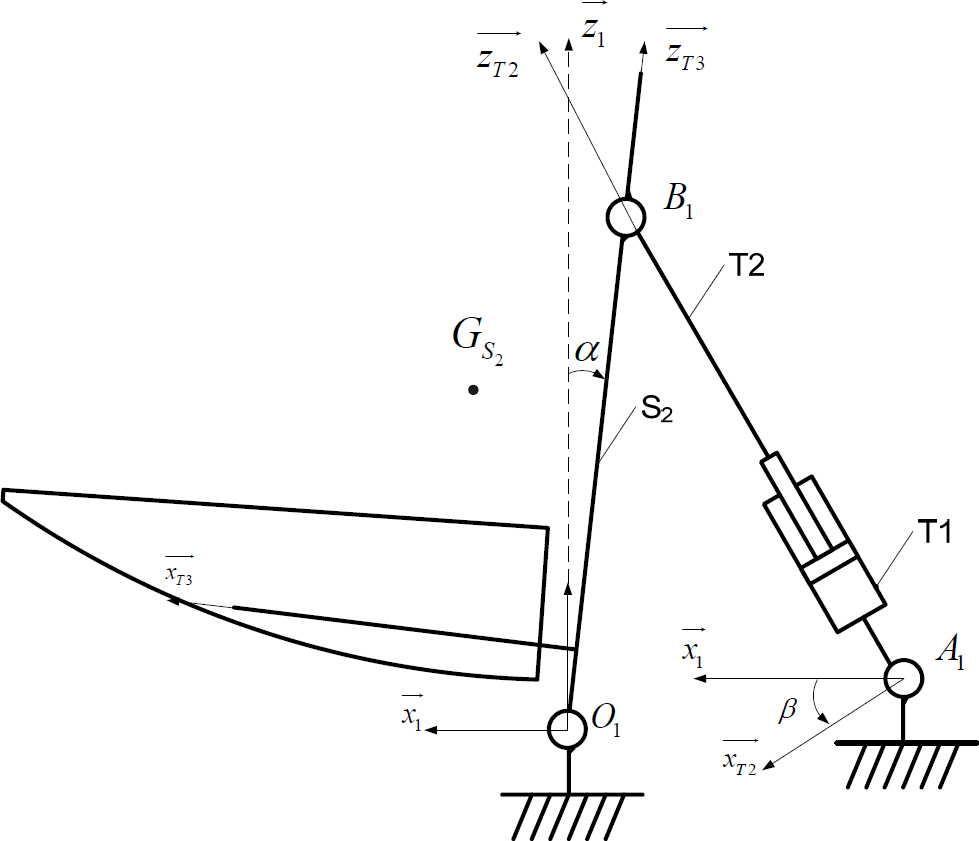
\includegraphics[width=.45\linewidth]{fig_13.png}
%\caption{Configuration plane du châssis\label{fig_13}}
%\end{figure}
%
%\question{Indiquer s'il est possible de déterminer, par une analyse statique globale, les différentes
%actions $\indice{N}{AV}$, $\indice{T}{AV}$, $\indice{N}{C}$, $\indice{T}{C}$, $\indice{N}{AR}$, $\indice{T}{AR}$. Justifier la réponse.}
%
%La modélisation plane de la \autoref{fig_13} est considérée dans la suite de cette partie.



\ifprof
\else
On considère qu'il y a roulement sans glissement au contact roue-sol. Les actions mécaniques du
sol sur chaque ensemble sont schématisées sur la \autoref{fig_13}; elles sont modélisées par un effort
normal ($\indice{N}{AV}$, $\indice{N}{C}$ ou $\indice{N}{AR}$) et un effort tangentiel de traction ($\indice{T}{AV}$, $\indice{T}{C}$ ou $\indice{T}{AR}$) appliqués aux
points $\indice{P}{AV}$, $\indice{P}{C}$ ou $\indice{P}{AR}$ (projections des points de contact roue-sol $P_i$ dans le plan médian $\left(O,\vect{x},\vect{z}\right)$).

\begin{figure}[H]
\centering
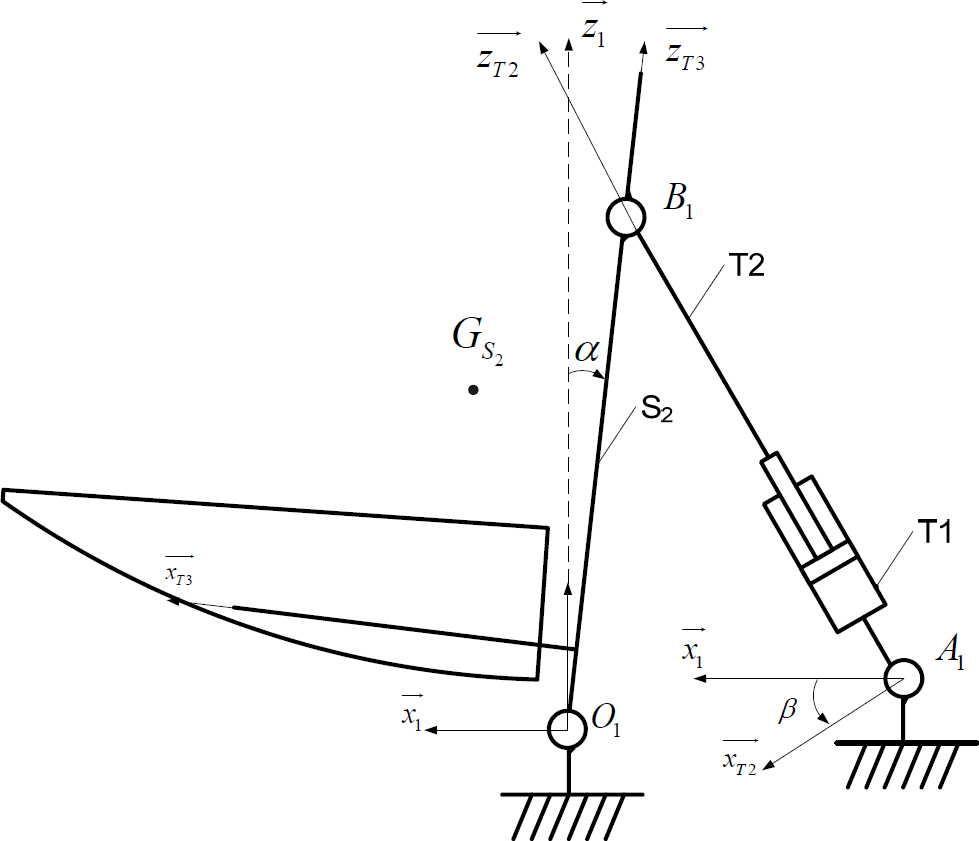
\includegraphics[width=.45\linewidth]{fig_13.png}
\caption{Configuration plane du châssis\label{fig_13}}
\end{figure}
\fi

\subsection{Comportement en pente et stabilité}
\begin{obj}
Dans cette sous-partie, on analyse le comportement en pente et la stabilité statique de la
plateforme.
\end{obj}


\ifprof
\else

On considère ici un sol plan dans le plan $\left(O,\vect{x},\vect{z}\right)$ et incliné d'un angle $\alpha$ par rapport à
l'horizontale (\autoref{fig_14}). La masse totale du système ROBOVOLC est répartie sur les trois
ensembles de la plateforme; les ensembles ENSAV et ENSAR ont la même masse
$\indice{m}{AV}=\indice{m}{AR}=m$ tandis que l'ensemble ENSC a une masse $m_C=M$. Les centres de gravité des
trois ensembles sont notés respectivement $\indice{G}{AV}$, $\indice{G}{C}$ et $\indice{G}{AR}$ ; ils sont indiqués sur la \autoref{fig_14}.

On a : $\vect{\indice{AG}{AV}}=\vect{\indice{OG}{C}}=\vect{\indice{DG}{AR}}=h\vect{z}$. 
Toutes les roues ont le même diamètre noté $D$.
On donne $D =\SI{300}{mm}$, $m =\SI{60}{kg}$, $M =\SI{80}{kg}$, $a =\SI{800}{mm}$, $b =\SI{200}{mm}$, $h =\SI{450}{mm}$.


\begin{figure}[H]
\centering
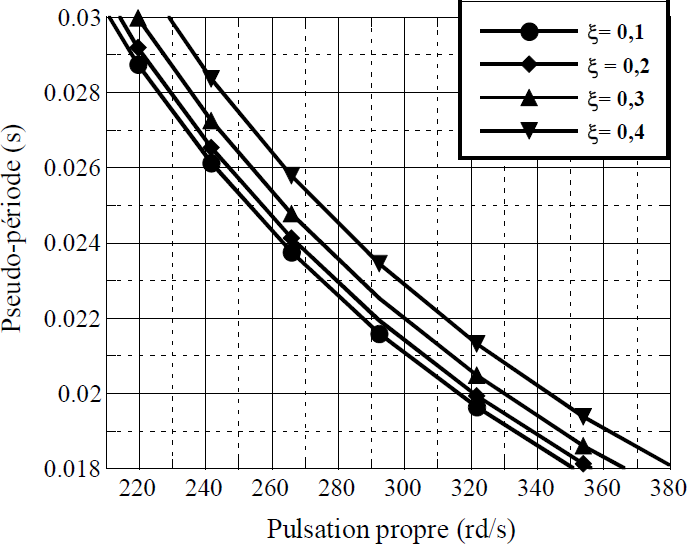
\includegraphics[width=.45\linewidth]{fig_14.png}
\caption{Configuration en pente \label{fig_14}}
\end{figure}
\fi

\question{Dans la configuration $\alpha = 0\degres$ (pente nulle), justifier la répartition des efforts normaux
suivante :  $\indice{N}{AV}= \indice{N}{AR}=mg$, $N_C=Mg$.}
\ifprof
\begin{corrige}
Par symétrie du système, on peut commencer par remarquer que le centre de gravité du système est situé en $G_c$.
On isole tout l’ensemble en équilibre et on applique le Principe Fondamental de Statique. 
\begin{itemize}
\item Le Théorème de la Résultante projeté sur $\vect{z}$ se traduit par : $\indice{N}{AV}+N_C+\indice{N}{AR}-(M+2m)g=0$.
\item Le Théorème du Moment Statique est appliqué au point $P_c$ en projection sur $\vect{y}$ se traduit par : $a\indice{N}{AV} - a \indice{N}{AR}=0$.
\end{itemize}
Ensuite, par identification, on obtient $\indice{N}{AV}=\indice{N}{AR}=mg$ et $N_C = Mg$.

\end{corrige}
\else
\fi

\question{Déterminer, en fonction des données géométriques, la hauteur $h$ limite des centres de
gravité avant basculement du système sur une pente inclinée d'un angle $\alpha$. En déduire la valeur
limite de $h$ à respecter pour satisfaire le cahier des charges, puis faire l'application numérique et
conclure. On donne $\tan (50\degres)\simeq 1,2$ .}
\ifprof
\begin{corrige}
On commence par étudier les configurations possibles de basculement. 

\begin{figure}[H]
\centering
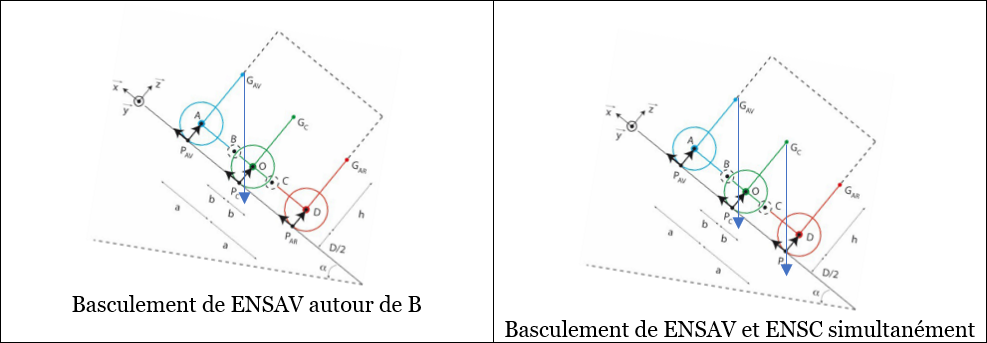
\includegraphics[width=.85\linewidth]{q13.png}
\end{figure}

Le basculement débutera donc obligatoirement par le basculement de la partie avant du véhicule.
A l’aide de considérations graphiques, il est possible de dire que le basculement débutera lorsque les efforts de pesanteur sur ENSAV seront « à droite » de B.

\begin{figure}[H]
\centering
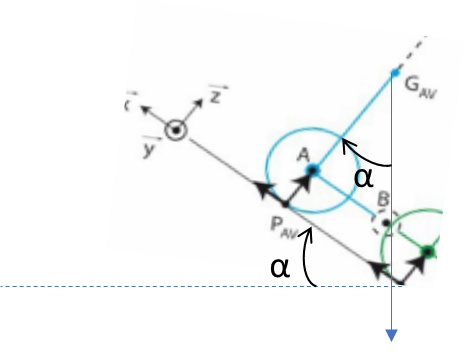
\includegraphics[width=.45\linewidth]{q13_02.png}
\end{figure}


La situation limite de basculement est tracée ci-contre (l’effort de pesanteur passe par le point $B$).
On lit directement sur la figure en utilisant les données du schéma : $\tan\alpha = \dfrac{AB}{\indice{AG}{AV}}= \dfrac{a-b}{h}$

La hauteur limite des centres de gravité avant basculement dans une pente $\alpha$ est donc :
$\indice{h}{lim}=\dfrac{a-b}{\tan \alpha}$.

Le cahier des charges impose de monter des pentes de 50\degres, on obtient donc une hauteur limite $h$ après application numérique : $\indice{h}{lim} = \dfrac{0,6}{1,2}=\SI{0,5}{m}$.


Deuxième méthode : 
En isolant ENSAV et en appliquant le Principe Fondamental de la Statique, on pourra résoudre sachant qu’à la limite du basculement, $\indice{N}{AV}$ est connu et vaut 0.
 

\begin{itemize}
\item Théorème de la résultante sur $\vect{x}$: $\indice{T}{AV}+\indice{X}{ensc-ensav}-mg \sin \alpha=0$
\item Théorème de la résultante sur $\vect{z}$: $\indice{N}{AV}+\indice{Y}{ensc-ensav}-mg \cos \alpha=0$
\item Théorème du Moment sur $\vect{y}$ au point B : $-mgh \sin\alpha+mg(a-b)\cos\alpha -\indice{N}{AV} (a-b)-\indice{T}{AV} h=0$.
\end{itemize}

A la limite du basculement, les efforts sur la roue avant sont nuls et l’équation de moment devient :
$-mg\indice{h}{lim}  \sin\alpha + mg(a-b) \cos \alpha =0$ soit encore $\indice{h}{lim} = \dfrac{a-b}{\tan \alpha}$.


\end{corrige}
\else
\fi


\ifprof
\else
Dans la question suivante, on fait l'hypothèse (notée HYP1) de limite de glissement au contact
entre le sol et la paire de roues de l'ensemble ENSC le plus chargé. On note $\mu$ le coefficient
de frottement.
\fi

\question{Montrer que l'hypothèse HYP1 permet de calculer l'ensemble des efforts de contact roue-sol
 dans la configuration $\alpha \neq 0$ (le calcul n'est pas demandé). Quelle équation permet de
démontrer que $\indice{N}{AV}\neq\indice{N}{AR}$ dans cette configuration ?}
\ifprof
\begin{corrige}
Dans le cas où les 3 coefficients de frottement ne sont pas connus, on a démontré qu’il n’était pas possible de résoudre, car il nous manquait une équation.
Avec l’HYP1, la résolution devient possible puisque l’on rajoute une équation de comportement.
L’écriture du Théorème du Moment Statique appliqué au point $P_c$  permet de démontrer l’inégalité $\indice{N}{AV}\neq\indice{N}{AR}$.

\end{corrige}
\else
\fi

%\subsection{Franchissement d'un obstacle}
%
%\begin{obj}
%Dans cette sous-partie, on étudie le franchissement par ROBOVOLC d'un obstacle en
%analysant les différentes phases du franchissement en terme d'efforts sur les roues.
%\end{obj}
%
%L'obstacle est matérialisé par une marche (pente verticale) de hauteur $H$ dans le plan $\left(O,\vect{x},\vect{z}\right)$,
%$\vect{z}$ correspondant à la verticale \autoref{fig_15}.
%On s'intéresse particulièrement aux trois phases représentées sur la \autoref{fig_15}, correspondant à la
%montée de chacun des trois ensembles (respectivement ENSAV pour la phase 1, ENSC pour la
%phase 2 et ENSAR pour la phase 3) le long de l'obstacle.
%
%Les notations utilisées (géométrie, actions mécaniques) sont similaires à celles de la sous-partie
%précédente.
%
%\begin{figure}[H]
%\centering
%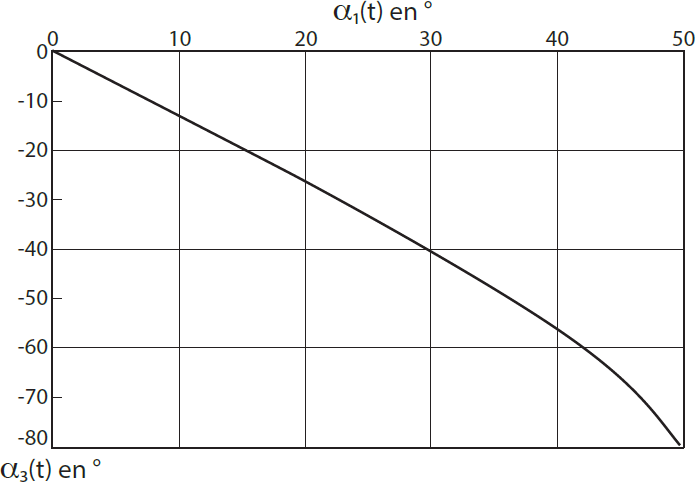
\includegraphics[width=.45\linewidth]{fig_15.png}
%\caption{Schématisation de l'obstacle et des phases de son franchissement\label{fig_15}}
%\end{figure}
%
%
%% Q3.8
%\question{Pour chacune des trois phases, donner les deux équations obtenues par le théorème de la
%résultante statique selon $\vect{x}$ et $\vect{z}$. Les autres équations de statique ne sont pas demandées.}
%
%Sous l'hypothèse (notée HYP2) de \textbf{limite de glissement pour la paire de roues montant le long
%de l'obstacle}, l'ensemble des équations de statique donne accès aux valeurs des efforts de
%contact roue-sol. On représente dans l'Annexe 2 les diagrammes d'évolution simulée de ces efforts
%au cours du franchissement de l'obstacle, pour une hauteur de l'obstacle $H =\SI{400}{mm}$ et un
%coefficient de frottement roue-sol $\mu = 0,5$ ou $\mu = 2$.
%
%% Q3.9
%\question{Identifier les plages temporelles des diagrammes où ont lieu chacune des phases 1, 2 et 3.
%Indiquer également à quoi correspondent les autres phases des diagrammes, et préciser l'origine
%des sauts d'effort observés.}
%
%% Q3.10
%\question{Expliquer pourquoi, sous l'hypothèse HYP2, il n'est pas possible de franchir l'obstacle
%avec un coefficient de frottement $\mu = 0,5$.}
%
%
%\subsection{Sélection des couples optimaux}
%
%\begin{obj}
%Dans cette sous-partie, on met en place un algorithme de calcul des couples optimaux à
%appliquer à chaque roue.
%\end{obj}
%
%
%Les actions extérieures exercées sur chaque roue (ou chaque paire de roues) sont représentées
%sur la \autoref{fig_16} :
%\begin{itemize}
%\item $N$ est la composante d'effort normale au contact roue-sol ;
%\item $T$ est la composante d'effort tangentielle au contact roue-sol ;
%\item $C_m$ est le couple moteur ;
%\item $M_r=k N$ est le couple résistant de frottement (résistance au roulement) avec $k$ un
%coefficient constant dépendant de la géométrie de la surface de contact roue-sol et des
%caractéristiques matériau de la roue et du sol.
%\end{itemize}
%
%Chaque roue est supposée rigide et est assimilée à un cylindre parfait.
%
%\begin{figure}[H]
%\centering
%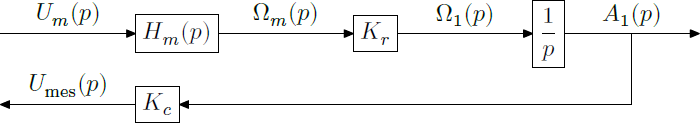
\includegraphics[width=.45\linewidth]{fig_16.png}
%\caption{Schématisation des actions extérieures sur une roue\label{fig_16}}
%\end{figure}
%
%\question{Donner la relation entre le couple moteur $C_m$ et les autres actions extérieures.}
%
%En lien avec l'évolution des efforts donnée dans l'Annexe 2, on trace sur la\autoref{fig_17} l'évolution
%des couples $\indice{C}{m, AV}$, $\indice{C}{m,C}$ et $\indice{C}{m,AR}$ sur chaque paire de roues en fonction du temps lors du franchissement d'un obstacle de hauteur $H =\SI{400}{mm}$ et pour $\mu=2$.
%
%\begin{figure}[H]
%\centering
%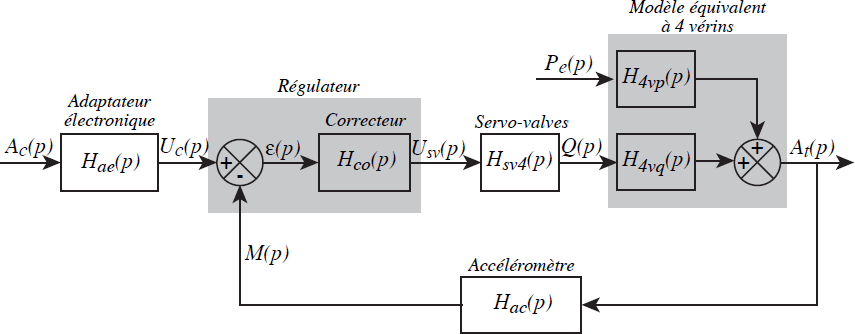
\includegraphics[width=.45\linewidth]{fig_17.png}
%\caption{Evolution du couple sur chaque paire de roues\label{fig_17}}
%\end{figure}
%
%
%% Q3.12
%\question{Conclure sur la valeur de couple à retenir pour le dimensionnement des moteurs, et
%remettre en cause l'utilisation de l'hypothèse HYP2 pour ce dimensionnement.}
%
%On cherche à présent la meilleure répartition du couple sur chaque roue, minimisant la puissance
%motrice tout en évitant le glissement.
%
%% Q3.13
%\question{Proposer un algorithme de répartition du couple sur chaque roue, qui serait une alternative
%à l'hypothèse HYP2 et permettrait de sélectionner des couples optimaux.}


\subsection{Asservissement en couple – contrôle de traction}

\begin{obj}
Dans cette sous-partie, on étudie l’asservissement en couple des moteurs utilisé pour
limiter le glissement. Le cahier des charges à respecter est le suivant :

\begin{center}
\begin{tabular}{ll}
\hline
\textbf{Critère} & \textbf{Valeur} \\ \hline \hline
Dépassement autorisé & inférieur à 5 \% \\ \hline
Temps de réponse à 5 \% & inférieur à \SI{9}{ms} \\ \hline
\end{tabular}
\end{center}

\end{obj}


\ifprof
\else

La structure d’asservissement proposée est composée de deux correcteurs utilisés simultanément :
un correcteur de boucle de retour (nommé $C_{\text{fb}}( p)$) et un correcteur de boucle d'anticipation
(nommé $C_{\text{ff}}( p)$ ). L’étude menée ici concerne le comportement du système avec cette structure
de correction.
Le schéma d'asservissement est donné sur la \autoref{fig_18}.

\begin{figure}[H]
\centering
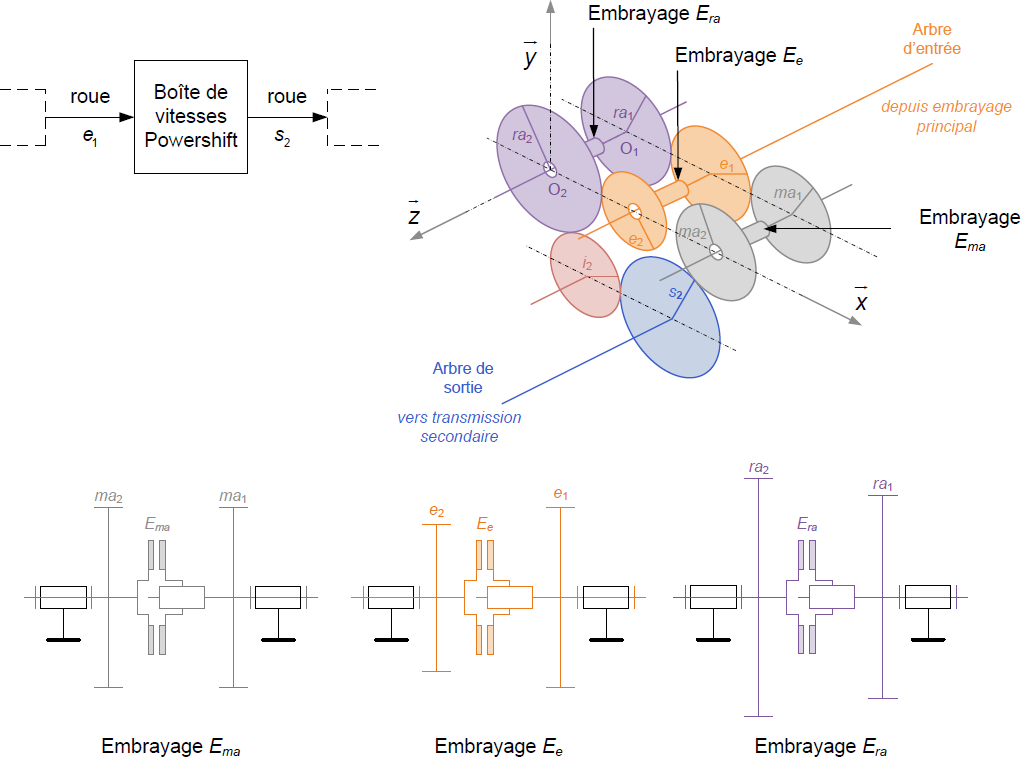
\includegraphics[width=.45\linewidth]{fig_18.png}
\caption{Schématisation de l'asservissement en couple \label{fig_18}}
\end{figure}


Le bloc  $\indice{H}{mot} (p)$ représente un moteur ayant pour fonction de transfert
$\indice{H}{mot} (p)=\dfrac{K_c}{K_c K_e+(R+Lp)( f +Jp)}$. Par identification, on trouve $\indice{H}{mot}= \dfrac{0,265}{0,4 p+200}$.
\fi


% Q3.14
\question{Énoncer, en justifiant, les hypothèses permettant de négliger les termes $L$ et $f$ pour
cette modélisation du moteur par une fonction de transfert du premier ordre.}
\ifprof
\begin{corrige}
Le modèle de connaissance est du second ordre. Or il nous est fourni un modèle du premier ordre. Cela signifie que le coefficient d’amortissement $\xi$ est supérieur à 1. Par conséquent la fonction de transfert du second ordre peut s’écrire comme un produit de 2 premiers ordres.
On a alors :

$\indice{H}{mot} (p)=\dfrac{K_c}{K_c K_e+Rf}\dfrac{1}{1+\dfrac{RJ+Lf}{K_c K_e+Rf} p+\dfrac{LJ}{K_c K_e+Rf} p^2}$.
 
Si le coefficient de frottement est très faible (le couple dû aux frottements visqueux est très faible devant le couple électromagnétique), alors on peut considérer $f \simeq 0$.
On a alors :
$\indice{H}{mot} (p)=\dfrac{1}{K_e} \dfrac{1}{1+\dfrac{RJ}{K_c K_e} p+\dfrac{LJ}{K_c K_e} p^2}$

L’inductance $L$ étant généralement faible (la tension aux bornes de l’inductance faible vis-à-vis des tensions électriques présentes dans le montage), on peut considérer $L \simeq 0$.
Donc, on retrouve bien un modèle simplifié du 1er ordre tel que proposé.
 

\end{corrige}
\else
\fi

On néglige dans un premier temps la boucle d'anticipation ($\indice{C}{ff} =0$) et on prend
$\indice{C}{fb}( p)=\indice{K}{fb}+\dfrac{\indice{I}{fb}}{p}$.

% Q3.15
\question{Déterminer la fonction de transfert en boucle fermée.}
\ifprof
\begin{corrige}
$\indice{H}{mot} (p)=\dfrac{0,265}{0,4p+200}=\dfrac{\dfrac{0,265}{200}}{1+\dfrac{0,4}{200} p}=\dfrac{K}{1+\tau p}$.

$\dfrac{C_S (p)}{C_C (p)} = \dfrac{\indice{C}{fb} (p) \indice{H}{mot} (p)}{1+\indice{C}{fb} (p) \indice{H}{mot} (p) }=\dfrac{1+\dfrac{\indice{K}{fb}}{\indice{I}{fb}}  p}{1+\dfrac{K\indice{K}{fb}+1}{K\indice{I}{fb}} p+\dfrac{\tau}{K\indice{I}{fb}} p^2}$.
\end{corrige}
\else
\fi

La \autoref{fig_19} représente l'évolution du dépassement et du temps de réponse à 5\% en fonction du
coefficient d'amortissement $\zeta$.

% Q3.16
\question{En s'aidant de la \autoref{fig_19}, exprimer les conditions sur les paramètres $\indice{K}{fb}$ et $\indice{I}{fb}$ permettant de respecter le cahier des charges.}
\ifprof
\begin{corrige}
Les paramètres du modèle élaboré en question précédente sont les suivants :
$\xi=\dfrac{1}{2} \dfrac{K\indice{K}{fb}+1}{K\indice{I}{fb}} \sqrt{\dfrac{K\indice{I}{fb}}{\tau}}$
et
$\omega_0=\sqrt{\dfrac{K\indice{I}{fb}}{\tau}}$ .
Pour respecter le cahier des charges, il faut que $\xi \geq 0,7$ et $\omega_0\geq \SI{333}{rad/s}$.

\begin{center}
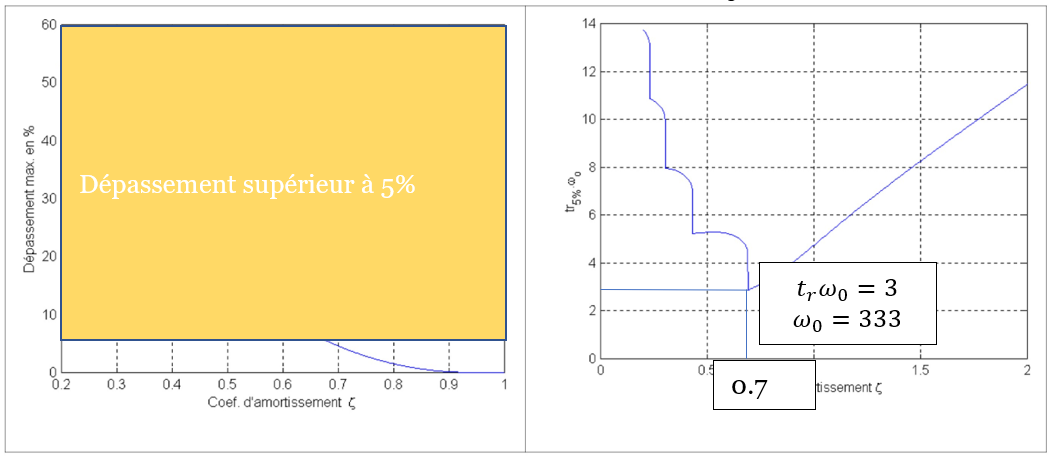
\includegraphics[width=.8\linewidth]{fig_19_cor.png}
\end{center}

Par une technique d’optimisation, un bon jeu de paramètres trouvé est $\indice{K}{fb} = 30$ et $\indice{I}{fb} = 200\times 10^3$.


%Les conditions traduites sur $\indice{I}{fb}$ et sur $\indice{K}{fb}$ donnent :
%$\dfrac{K}{\tau} \omega_0^2 \leq  \indice{I}{fb}$ soit $\indice{I}{fb} \geq 16,7 \times 10^5$
%$\dfrac{\dfrac{2\xi \indice{I}{fb}}-1}{K}\geq \indice{K}{fb}$ relation dont le résultat dépend de la valeur choisie pour $\indice{I}{fb}$.


\end{corrige}
\else
\fi

\ifprof
\else
\begin{figure}[H]
\centering
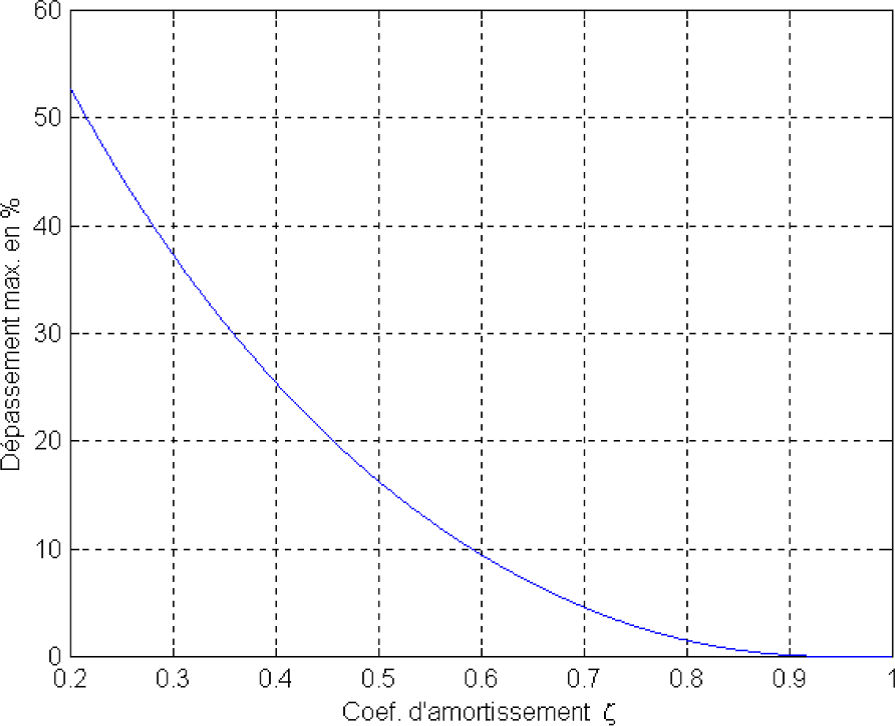
\includegraphics[width=.45\linewidth]{fig_19_a.png}
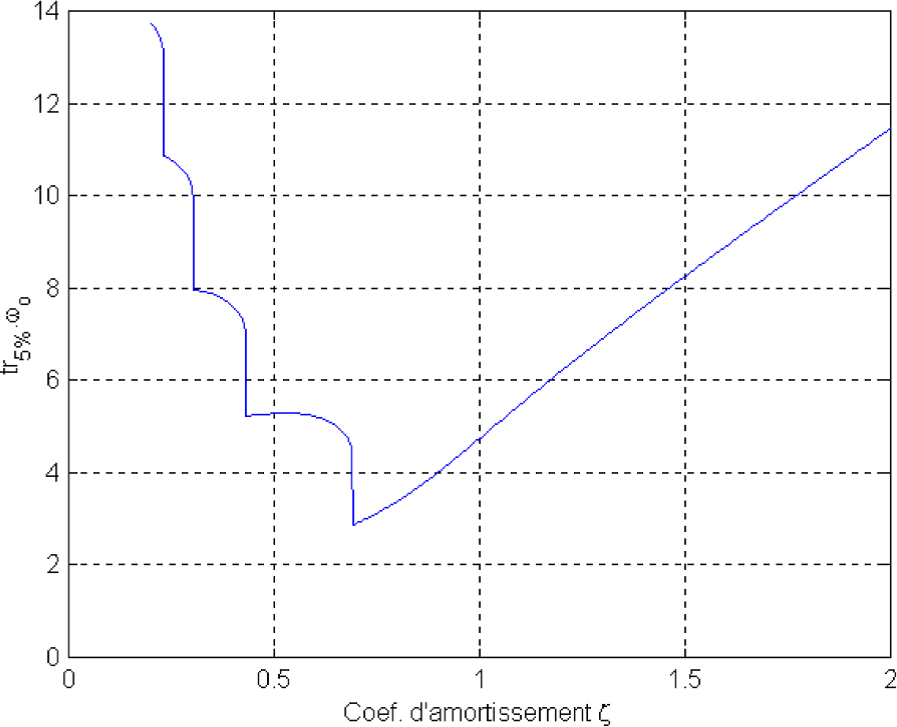
\includegraphics[width=.45\linewidth]{fig_19_b.png}
\caption{Dépassement et temps de réponse à 5\% en fonction de $\zeta$ \label{fig_19}}
\end{figure}


Par une technique d’optimisation, un bon jeu de paramètres trouvé est : $\indice{K}{fb}=30$ et $\indice{I}{fb}=200\times10^{3}$.
\fi

% Q3.17
\question{Calculer la valeur du dépassement et le temps de réponse.}
\ifprof
\begin{corrige}
Dans le cas avec le jeu de paramètre correct, on a : $\omega_0 \simeq \SI{365}{rad/s}$ et  $\xi \simeq 0,701$.

\begin{center}
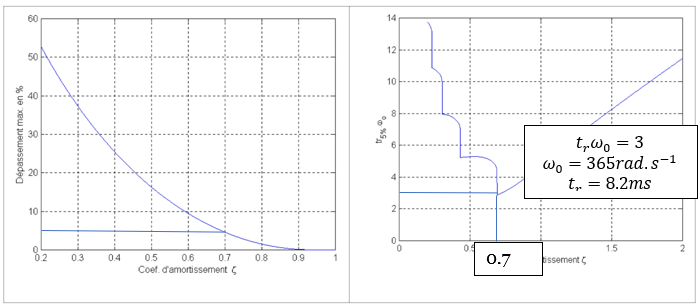
\includegraphics[width=.8\linewidth]{q19_cor.png}
\end{center}

Donc, d’après les courbes précédentes, on trouve : $t_{5\%} = \SI{8}{ms}$.

\end{corrige}
\else
\fi

% Q3.18
\question{Tracer sur le document réponse DR2 le diagramme de Bode asymptotique de la fonction
de transfert en boucle ouverte. Discuter des marges de gain et de phase.}
\ifprof
\begin{corrige}
La fonction de transfert en Boucle Ouverte s’exprime ainsi :

$\text{FTBO}(p)=\indice{C}{fb} (p) \indice{H}{mot} (p)=\left(30+\dfrac{200\times 10^3}{p}\right)\dfrac{0,265}{0,4p+200}$ 
$=265\left(1+\dfrac{p}{6667}\right) \left(\dfrac{1}{1+\dfrac{p}{500}}\right)$.

\begin{center}
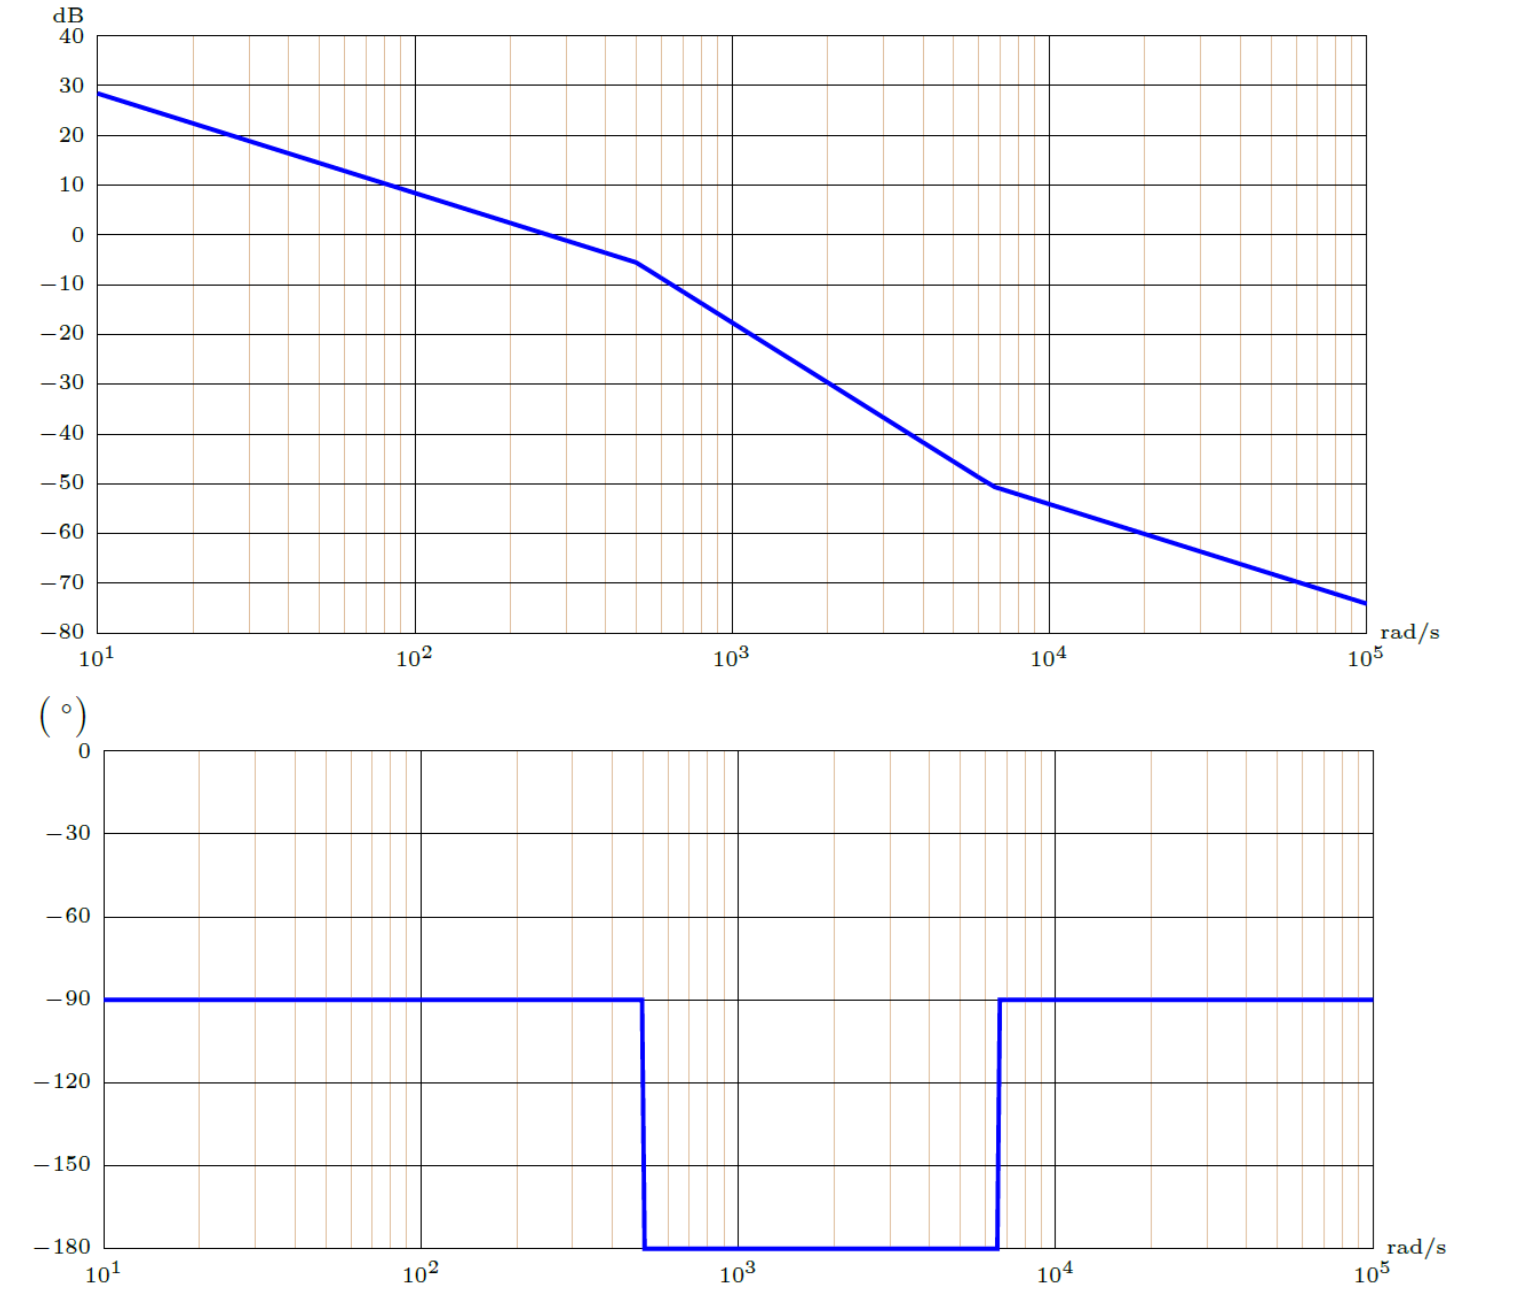
\includegraphics[width=.8\linewidth]{q19_bode.png}
\end{center}

La marge de gain est infinie (ou non définie) car la phase n’atteint jamais $-180\degres$.

La marge de phase est nécessairement positive, car la phase est strictement supérieure à $-180\degres$. Donc le système est bien stable en boucle fermée.
 


\end{corrige}
\else
\fi


On considère à présent la structure d'asservissement complète, avec le correcteur $\indice{C}{ff} (p)$.

% Q3.19
\question{Exprimer la fonction de transfert en boucle fermée du système en fonction de $\indice{H}{mot}( p)$ ,
$\indice{C}{fb} (p)$ et $\indice{C}{ff} (p)$.}
\ifprof
\begin{corrige}
$$
\dfrac{C_S (p)}{C_C (p)}= \left(1+\dfrac{\indice{C}{ff} (p)}{\indice{C}{fb} (p)}\right) \left(\dfrac{\indice{H}{mot}(p) \indice{C}{fb} (p)}{1+\indice{H}{mot} (p)\indice{C}{fb} (p) }\right)
$$
\end{corrige}
\else
\fi

% Q3.20
\question{Que se passe-t-il si le correcteur vaut $\indice{C}{ff} (p)= \dfrac{1}{\indice{H}{mot} (p)}$ ? Quel est l’intérêt et le risque ?}
\ifprof
\begin{corrige}
En admettant que l’on puisse réaliser un tel système (en fait, le système étant composé d’un gain et d’un dérivateur pur, il faudrait rajouter du filtrage afin d’avoir un système causal), on obtient après simplification :
 
$\dfrac{C_S (p)}{C_C (p)}=\left(1+\dfrac{1}{\indice{H}{mot}\indice{C}{fb} (p)}\right)\left(\dfrac{\indice{H}{mot} (p)\indice{C}{fb} (p))}{1+\indice{H}{mot} (p)\indice{C}{fb} (p)}\right)=1$

L’intérêt théorique d’un tel système est donc évident puisqu’il s’agit d’un système dont la réponse correspond parfaitement à la consigne.
Cependant, pour y parvenir, il faut parfaitement maîtriser les paramètres du modèle du moteur $\indice{H}{mot} (p)$.

Un risque est donc de ne pas avoir un modèle suffisamment précis de $\indice{H}{mot} (p)$ et donc d’avoir des réactions imprévisibles et non désirées du correcteur.

Un autre  écart entre la théorie et la réalisation pratique du correcteur  est lié à la saturation de la commande. Un tracé de la réponse du système à un échelon de commande réalisé avec le correcteur théorique (modèle fourni dans ce dossier) montre la commande théorique du système (ci-dessous).

\begin{center}
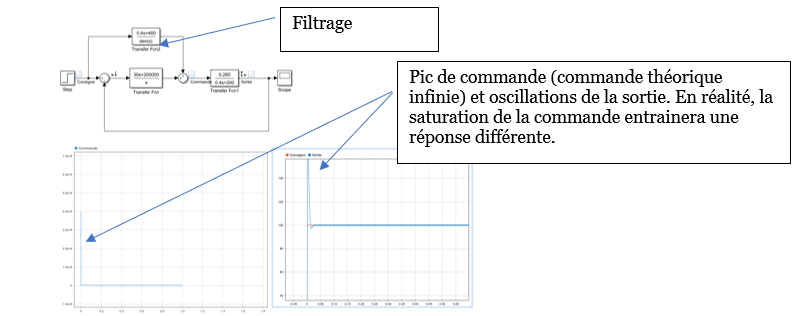
\includegraphics[width=.8\linewidth]{q21_cor.png}
\end{center}



\end{corrige}
\else
\fi

Pour une fonction de transfert $\indice{C}{fb} (p)$ fixée, on considère le correcteur $\indice{C}{ff}(p)$ comme un gain
proportionnel variable. Les courbes de réponse pour différentes valeurs de ce gain proportionnel
sont données dans l'Annexe 3.

% Q3.21
\question{Quelles conclusions peut-on en tirer sur l'effet du correcteur $\indice{C}{ff} (p)$?}
\ifprof
\begin{corrige}
 Ce correcteur à tendance à améliorer la rapidité sans trop dégrader la stabilité. Les critères de rapidité (temps de réponse à 5\%) et de stabilité (dépassement autorisé) sont respectés, voire même améliorés pour $\indice{C}{ff}  = 100$.
\end{corrige}
\else
\fi
